\section{Experimental Evaluation}
\label{sec:experiments}

{\bf{Dataset: }} Our model is tested on the PASCAL VOC 2012 segmentation benchmark \citep{everingham2014pascal}, consisting of 20 foreground object classes and one background class. The original dataset contains $1,464$, $1,449$, and $1,456$ images for training, validation, and testing, respectively. The dataset is augmented by the extra annotations provided by \citep{hariharan2011semantic}, resulting in $10,582$ training images. The performance is measured in terms of pixel intersection-over-union (IOU) averaged across the 21 classes. 

{\bf{Training: }} We adopt the simplest form of piecewise training, decoupling the DCNN and CRF training stages, assuming the unary terms provided by the DCNN are fixed during CRF training. 

For DCNN training we employ the VGG-16 netwok which has been pre-trained on ImageNet. We fine-tuned the VGG-16 network on the VOC 21-way classification task by stochastic gradient descent on the cross-entropy loss function. We use a mini-batch of 20 images and a learning rate of $0.001$ with ``step'' learning policy,  reducing the learning rate by 0.1 at every 2000 iterations. We use momentum of $0.9$ and a weight decay of $0.0005$. Since, as detailed in Sec.~2.2 our model has a stride of 8 in the last layer, the training labels are obtained by downsampling the ground truth segmentations by a factor of 8.

%a DCNN is first fine-tuned on the training set and then, as in the work of \citet{krahenbuhl2011efficient}  we cross-validate the 
  After the DCNN has been fine-tuned, we cross-validate the   parameters of the fully connected CRF model in \equref{eq:fully_crf} along the lines of \citet{krahenbuhl2011efficient};
 to avoid overfitting the validation set, the parameters $w^2$ and $\sigma_\gamma$ are fixed to be $3$ and the best values of $w^1$, $\sigma_\alpha$, and $\sigma_\beta$ are cross-validated on a small subset of the validation set (we use around 200 images).  

{\bf{Evaluation on Validation set: }} We conduct the majority of our evaluations on the validation set. As shown in \tabref{tb:valIOU}, the performance improves moderately as multi-scale features are added. The fully connected CRF yields a substantially larger boost in performance, in the order of about 4\%; the improvement - while using both CRFs and multi-scale DCNN features yields an additional improvement. 
We note that the original work of \citet{krahenbuhl2011efficient} improved the $27.6\%$
result of TextonBoost \citep{shotton2009textonboost} to $29.1\%$, which makes the  improvement we report here (from $59.8\%$ to $63.7\%$) all the more impressive - since we have also a {\emph{larger relative}} improvement. We can understand this as indicating how essential it has been to use  a CRF on top of DCNN features - which apparently were so loosely localized  that they would leave a large margin of improvement to the CRF. 

Turning to qualitative results, the effect of employing multi-scale features is visualized in \figref{fig:msBoundary}. The predicted object boundaries are refined, but   far from perfect. By contrast, employing a fully connected CRF significantly improves the results visually, especially along intricate object boundaries. We provide more visual comparisons between DeepLab-MSc and DL-MSc-CRF in \figref{fig:ValResults}.

\begin{table}
  \centering
  \begin{tabular}{c | c}
    Method      & mean IOU (\%) \\
    \hline
    DeepLab     & 59.80 \\
    DeepLab-MSc & 60.25 \\
    DeepLab-CRF & 63.74 \\
    DL-MSc-CRF  & 64.14 \\
  \end{tabular}
  \caption{Performance of our proposed models on the validation set. DeepLab-MSc: multi-scale features are added to DeepLab. DeepLab-CRF: combination of DeepLab and fully connected CRF. DL-MSc-CRF: combination of DeepLab-MSc and fully connected CRF}.
  \label{tb:valIOU}
\end{table}

\begin{figure}[ht]
  \centering
  \begin{tabular}{c c | c c}
      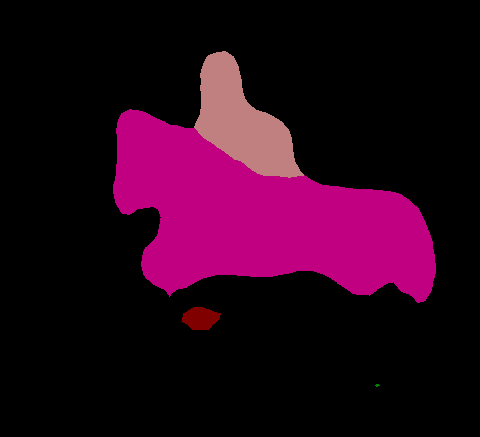
\includegraphics[height=0.14\linewidth]{fig/boundary_refine/vgg128noup_2007_000783.png} &
      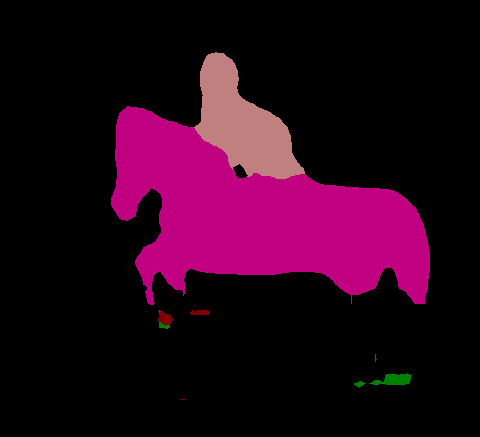
\includegraphics[height=0.14\linewidth]{fig/boundary_refine/vgg128ms_2007_000783.png} &
      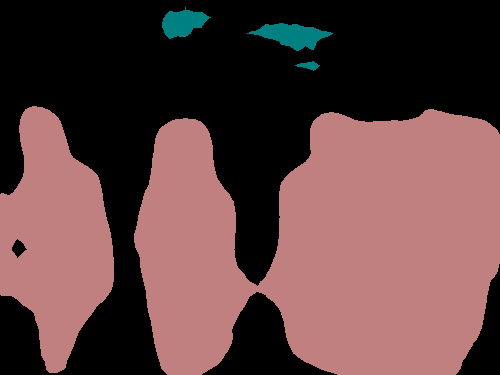
\includegraphics[height=0.14\linewidth]{fig/boundary_refine/vgg128noup_2007_001284.png} &
      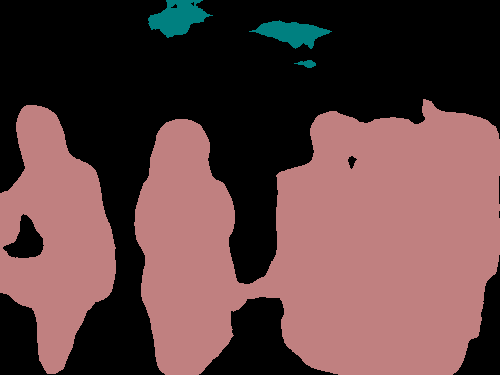
\includegraphics[height=0.14\linewidth]{fig/boundary_refine/vgg128ms_2007_001284.png} \\
      \hline
      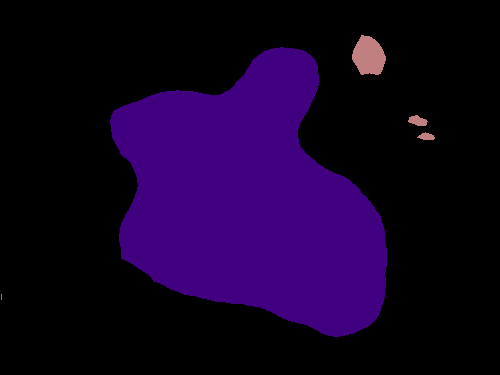
\includegraphics[height=0.12\linewidth]{fig/boundary_refine/vgg128noup_2007_001239.png} &
      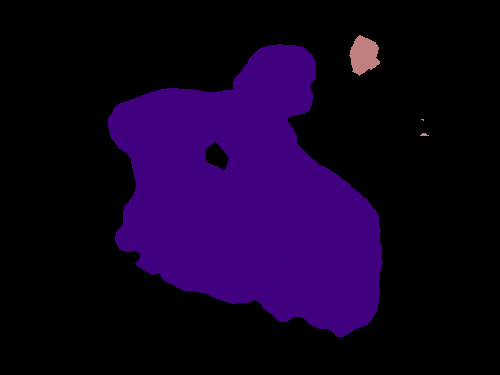
\includegraphics[height=0.12\linewidth]{fig/boundary_refine/vgg128ms_2007_001239.png} &
      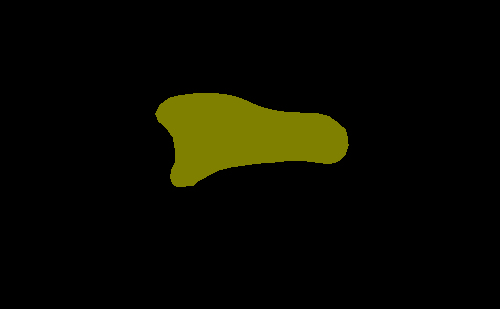
\includegraphics[height=0.12\linewidth]{fig/boundary_refine/vgg128noup_2007_001289.png} &
      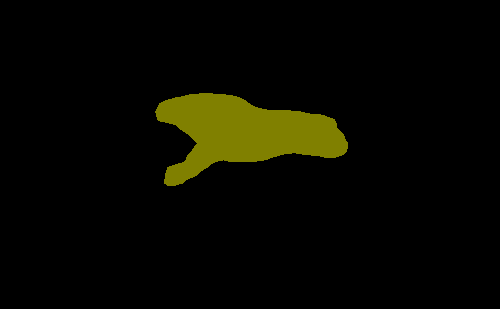
\includegraphics[height=0.12\linewidth]{fig/boundary_refine/vgg128ms_2007_001289.png} \\
      (a) & (b) & (a) & (b) \\ 
  \end{tabular}
  \caption{Incorporating multi-scale features improves the boundary segmentation. Our DeepLab-MSc (b) can slightly improve the boundary segmentation compared to DeepLab (a).}
  \label{fig:msBoundary}
\end{figure}


{\bf{Weighted loss: }} Weighting the loss function according to the class frequency has been employed, e.g. in \cite{mostajabi2014feedforward} to overcome the label imbalance problem. We have experimented with this idea by adjusting the loss function for one pixel to be $-\frac{1}{n_{x}} \log P(x)$, where $n_x$ is the frequency of class $x$ and $P$ is the prediction probability. Our experiments on VOC 2012 val set show that using a weighted loss function increases the mean class accuracy (the pixelwise accuracy averaged across classes) from $73.68\%$ to $88.81\%$. However, the mean IOU decreases a lot from $59.80\%$ to $41.77\%$. We found that many background pixels are labeled as foreground classes because the mislassifying the background class incurs a lower  loss, resulting in an increase of  the false positives rate of  foreground classes. This finding is inconsistent to \citet{mostajabi2014feedforward}. We suspect it is because they predict labels for superpixels while we employ sliding windows for pixel prediction.

{\bf{Mean Pixel IOU along Object Boundaries: }}
To quantify the improvement of different models, we evaluate the segmentation accuracy around object boundaries \citep{kohli2009robust, krahenbuhl2011efficient}. Specifically, we  use  the ``void'' label annotated in val set, which usually occurs around object boundaries. We compute the mean IOU for those pixels that are located within a narrow band (called trimap) of ``void'' labels. As shown in \figref{fig:IOUBoundary}, adding multi-scale features improves the accuracy slightly. On the other hand, refining the segmentation results by a fully connected CRF significantly improves the results around object boundaries. 

{\bf{Test set results: }} Having set our model choices on the validation set, we turn to evaluating our model, DeepLab-CRF\footnote{http://host.robots.ox.ac.uk:8080/anonymous/NTHWZK.html}, on the VOC 2012 test set. As shown in \tabref{tab:voc2012}, our model achieves performance of $66.4\%$ mean IOU, outperforming all the other state-of-the-art models. 

\begin{table*}[ht]\scriptsize
\setlength{\tabcolsep}{3pt}
%\hspace{-1.8cm}
\resizebox{\columnwidth}{!}{
\begin{tabular}{|c||c*{20}{|c}||c|}
\hline
Method         & bkg &  aero & bike & bird & boat & bottle& bus & car  &  cat & chair& cow  &table & dog  & horse & mbike& person& plant&sheep& sofa &train & tv   & mean \\
\hline\hline
DeepLab-CRF    &{\bf 92.1} & 78.4 & 33.1 & {\bf 78.2} & 55.6 & 65.3 & {\bf 81.3} & {\bf 75.5} & 78.6 & 25.3 & 69.2 & 52.7 & {\bf 75.2} & 69.0  & {\bf 79.1} & {\bf 77.6} & {\bf 54.7} & {\bf 78.3} & {\bf 45.1} & {\bf 73.3} & {\bf 56.2} & {\bf 66.4} \\ 
\hline
TTI-Zoomout-16 & 89.8 & {\bf 81.9} & {\bf 35.1} & {\bf 78.2} & {\bf 57.4} & 56.5 & 80.5 & 74.0 & {\bf 79.8} & 22.4 & {\bf 69.6} & {\bf 53.7} & 74.0 & {\bf 76.0} & 76.6 & 68.8 & 44.3 & 70.2 & 40.2 & 68.9 & 55.3 & 64.4 \\
FCN-8s         & -    & 76.8 & 34.2 & 68.9 & 49.4 & 60.3 & 75.3 & 74.7 & 77.6 & 21.4 & 62.5 & 46.8 & 71.8 & 63.9  & 76.5 & 73.9 & 45.2 & 72.4 & 37.4 & 70.9 & 55.1 & 62.2 \\
MSRA-CFM       & -    & 75.7 & 26.7 & 69.5 & 48.8 & {\bf 65.6} & 81.0 & 69.2 & 73.3 & {\bf 30.0} & 68.7 & 51.5 & 69.1 & 68.1  & 71.7 & 67.5 & 50.4 & 66.5 & 44.4 & 58.9 & 53.5 & 61.8 \\
\hline
 \end{tabular}
}
 \caption{Labeling IoU (\%) on the PASCAL VOC 2012 test set, using the trainval set for training.}
 \label{tab:voc2012}
\end{table*}



% \begin{figure}[ht]
%   \centering
%   \begin{tabular}{c c c | c c}
%     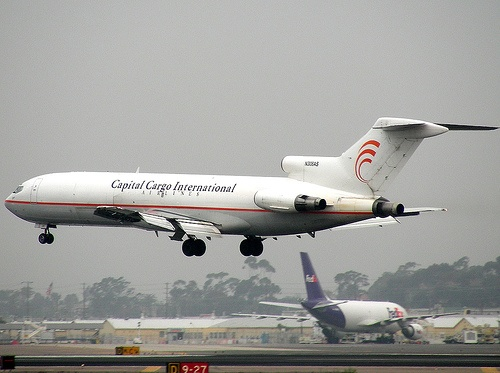
\includegraphics[height=0.12\linewidth]{fig/img/2007_002266.jpg} &
%     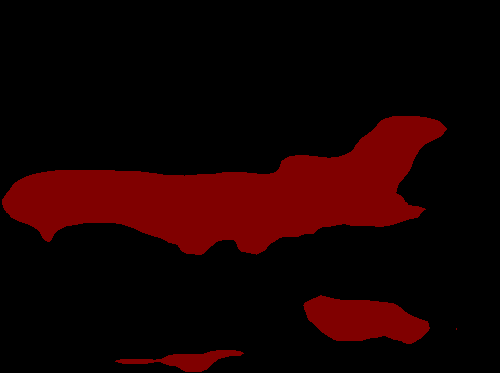
\includegraphics[height=0.12\linewidth]{fig/fcn8s/2007_002266.png} &
%     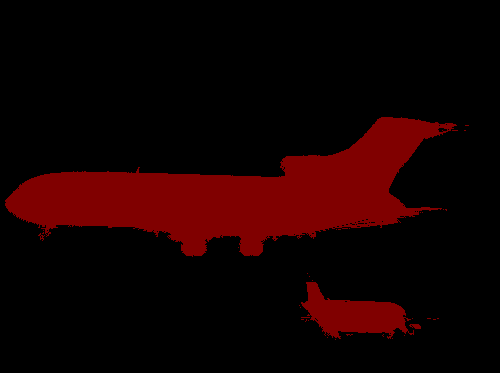
\includegraphics[height=0.12\linewidth]{fig/res_crf/2007_002266.png} &
%     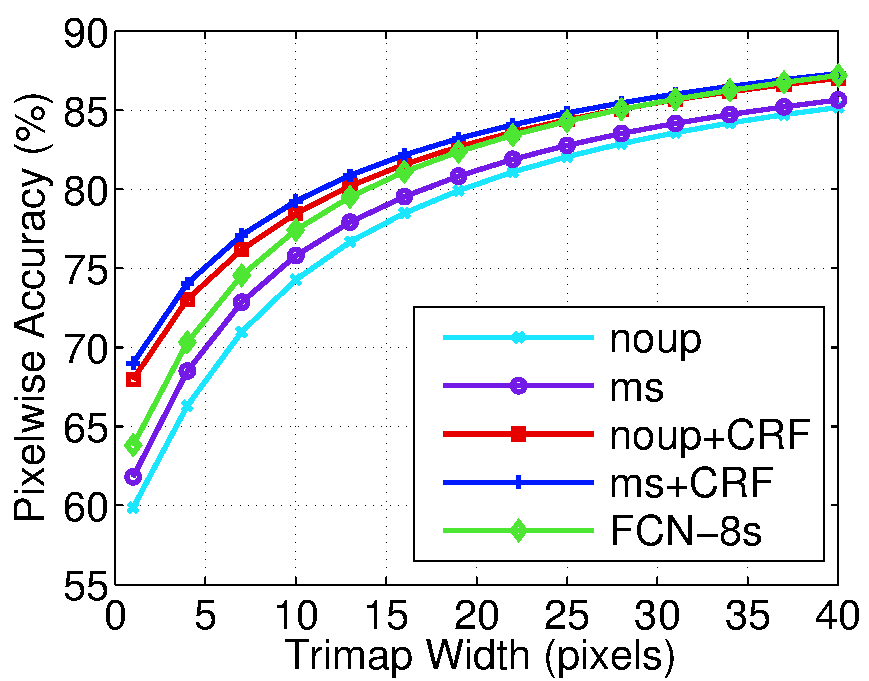
\includegraphics[height=0.12\linewidth]{fig/SegPixelAccWithinTrimap_Berkeley.pdf} &
%     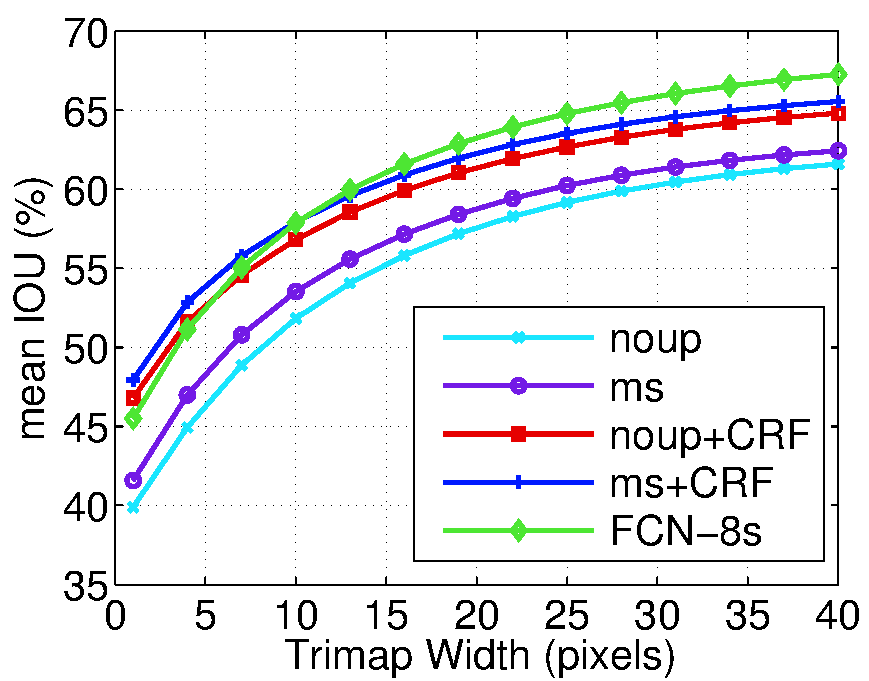
\includegraphics[height=0.12\linewidth]{fig/SegPixelIOUWithinTrimap_Berkeley.pdf} \\
%     (a) & (b) & (c) & (d) & (e)
%   \end{tabular}
%   \caption{(Left) Some comparisons with FCN-8S: (a) image; (b) FCN-8S; (c)
%     ms-crf. (d) Segmentation accuracy (pixelwise accuracy) within trimap. (e)
%     Segmentation accuracy (mean IOU) within trimap. {\color{red} TODO: change
%       legend. HELP: I cannot make them equally spaced....}} 
%   \label{fig:IOUBoundary}
% \end{figure}

\begin{figure}
\centering
\resizebox{\columnwidth}{!}{
  \begin{tabular} {c c c}
%    \hspace{-0.5cm}\raisebox{2cm}
    \raisebox{1.7cm} {
    \begin{tabular}{c c}
      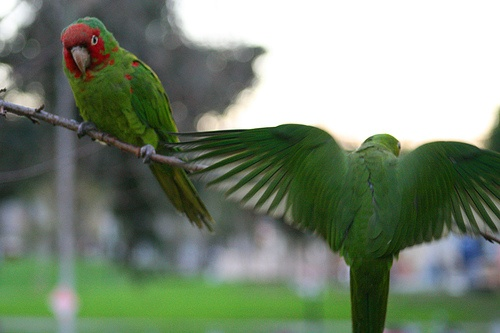
\includegraphics[height=0.1\linewidth]{fig/trimap/2007_000363.jpg} &
      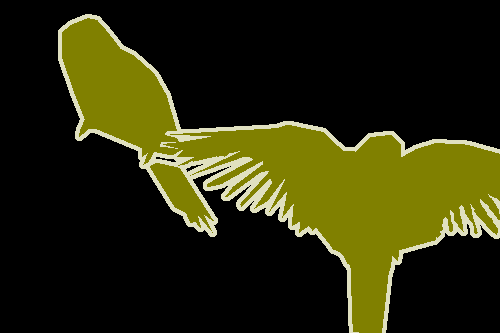
\includegraphics[height=0.1\linewidth]{fig/trimap/2007_000363.png} \\
      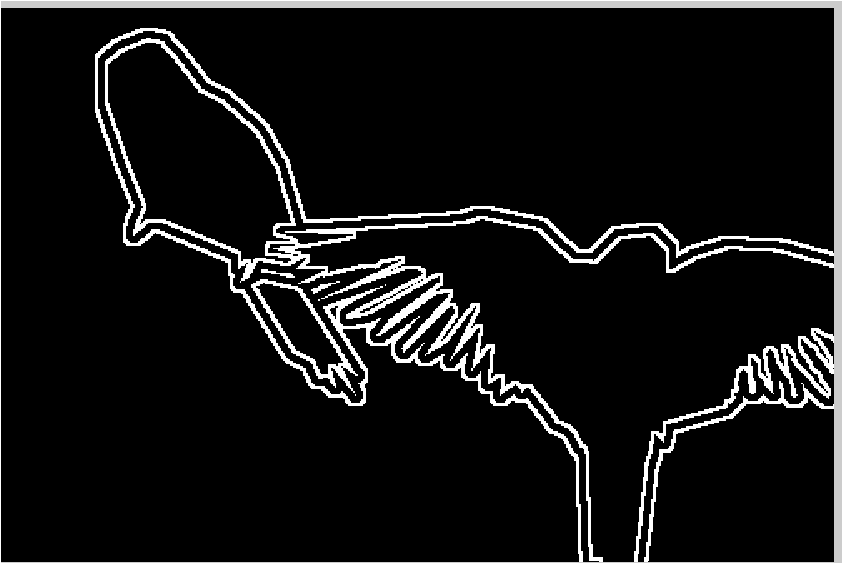
\includegraphics[height=0.1\linewidth]{fig/trimap/TrimapWidth2.pdf} &
      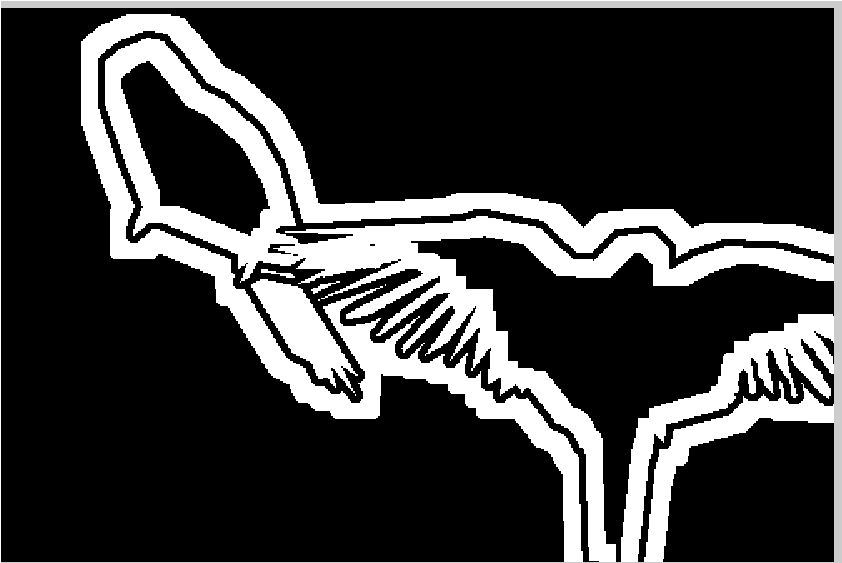
\includegraphics[height=0.1\linewidth]{fig/trimap/TrimapWidth10.pdf} \\
    \end{tabular} } &
    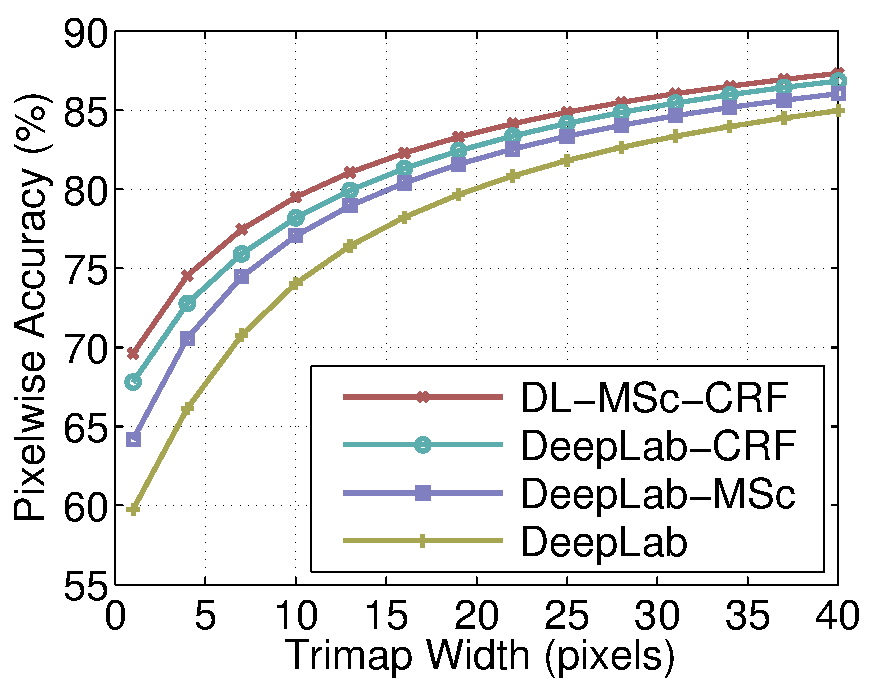
\includegraphics[height=0.25\linewidth]{fig/SegPixelAccWithinTrimap.pdf} &
    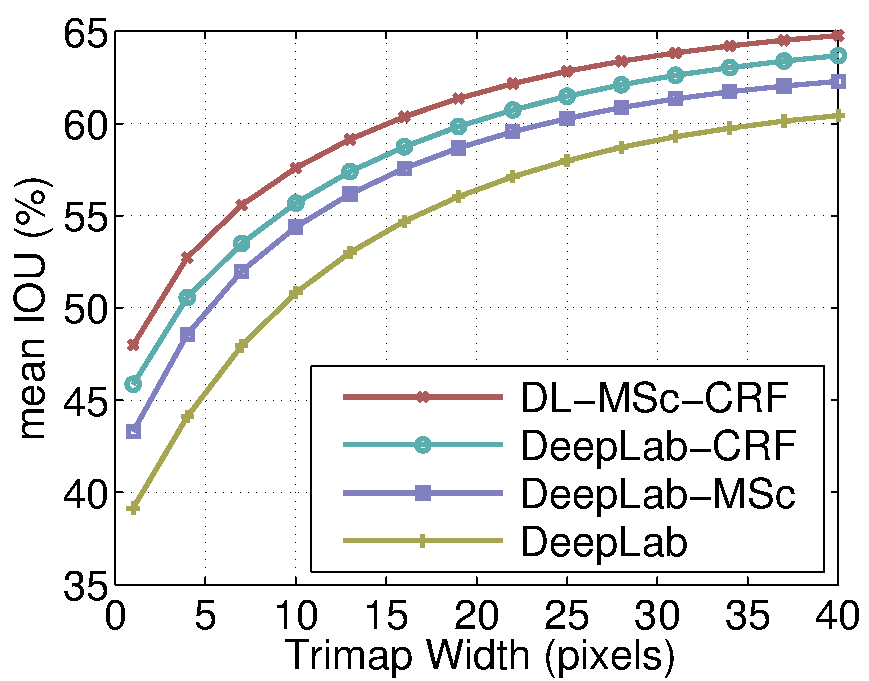
\includegraphics[height=0.25\linewidth]{fig/SegPixelIOUWithinTrimap.pdf} \\
    (a) & (b) & (c) \\
   \end{tabular}
}
  \caption{(a) Some trimap examples (top-left: image. top-right: ground-truth. bottom-left: trimap of 2 pixels. bottom-right: trimap of 10 pixels). Quality of segmentation result within a band around the object boundaries for the proposed methods. (b) Pixelwise accuracy. (c) Pixel mean IOU. 
    }  
  \label{fig:IOUBoundary}
\end{figure}


\begin{figure}[!htbp]
  \centering
  %\vspace{-1.cm}
  \scalebox{0.82} {
  \begin{tabular}{c c c | c c c}
    %\addtolength{\tabcolsep}{-6.5pt}
    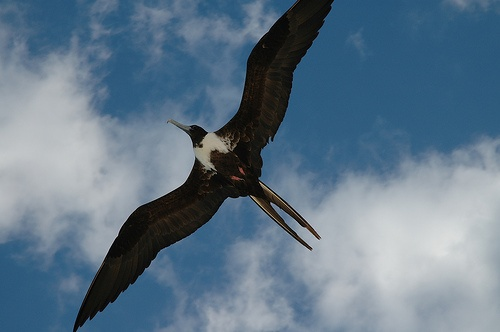
\includegraphics[height=0.12\linewidth]{fig/img/2007_002094.jpg} &
    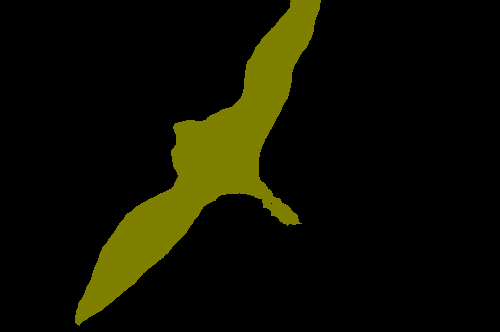
\includegraphics[height=0.12\linewidth]{fig/res_none/2007_002094.png} &
    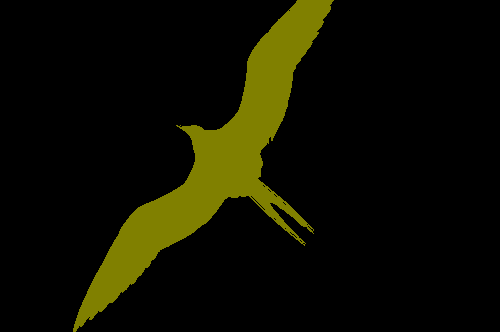
\includegraphics[height=0.12\linewidth]{fig/res_crf/2007_002094.png} &
    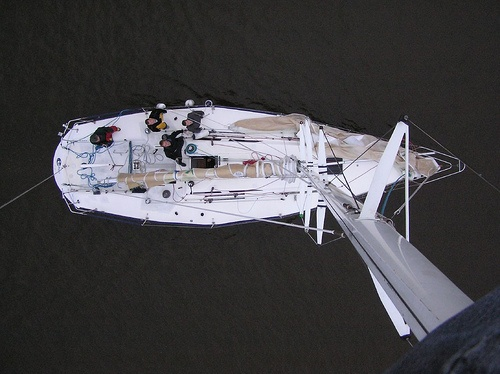
\includegraphics[height=0.12\linewidth]{fig/img/2007_002719.jpg} &
    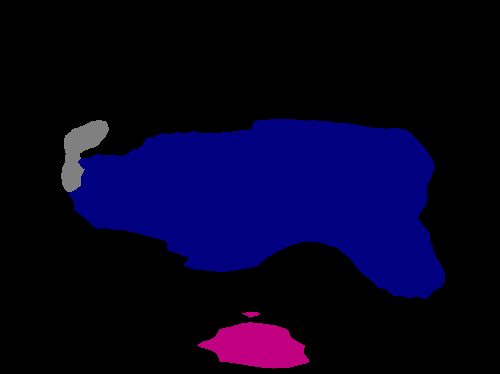
\includegraphics[height=0.12\linewidth]{fig/res_none/2007_002719.png} &
    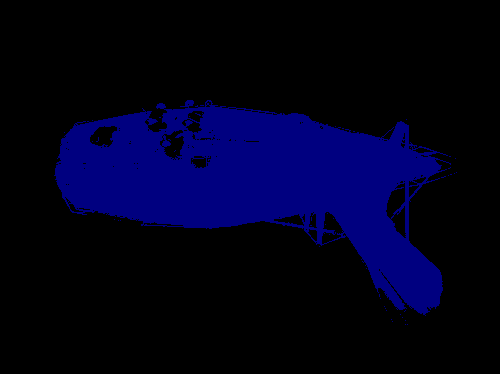
\includegraphics[height=0.12\linewidth]{fig/res_crf/2007_002719.png} \\
    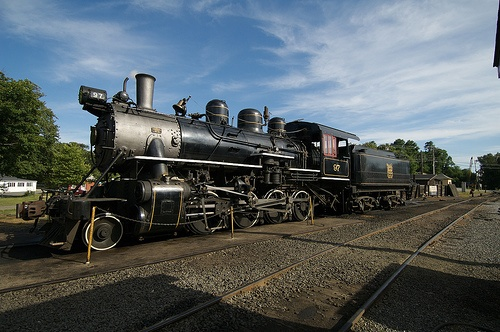
\includegraphics[height=0.12\linewidth]{fig/img/2007_003957.jpg} &
    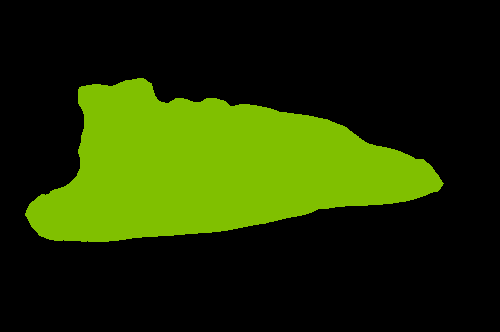
\includegraphics[height=0.12\linewidth]{fig/res_none/2007_003957.png} &
    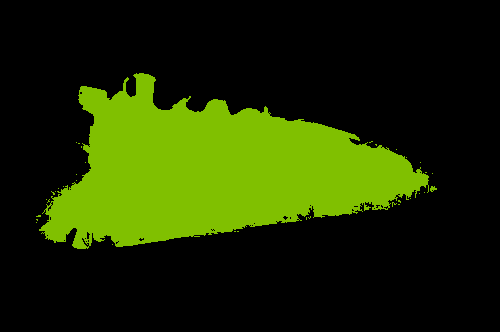
\includegraphics[height=0.12\linewidth]{fig/res_crf/2007_003957.png} &
    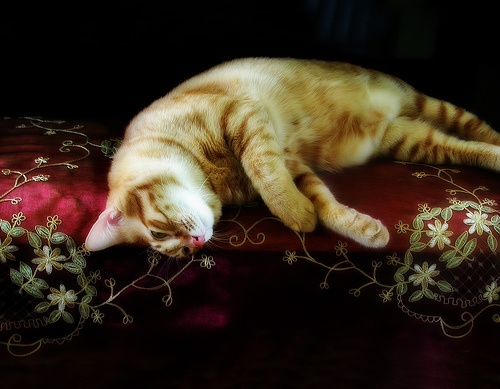
\includegraphics[height=0.12\linewidth]{fig/img/2007_003991.jpg} &
    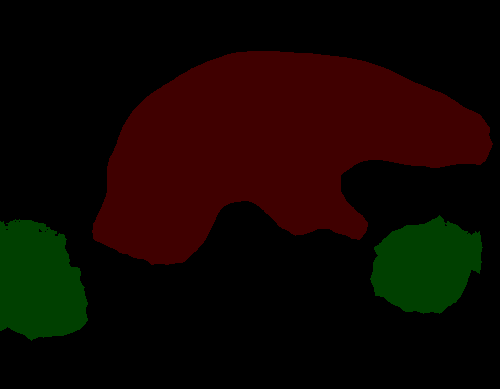
\includegraphics[height=0.12\linewidth]{fig/res_none/2007_003991.png} &
    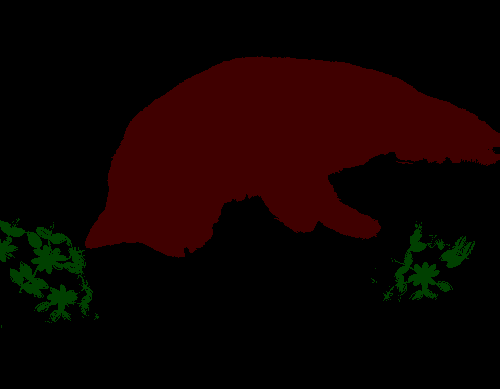
\includegraphics[height=0.12\linewidth]{fig/res_crf/2007_003991.png} \\
    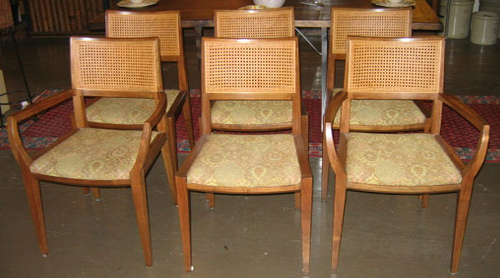
\includegraphics[height=0.10\linewidth]{fig/img/2008_001439.jpg} &
    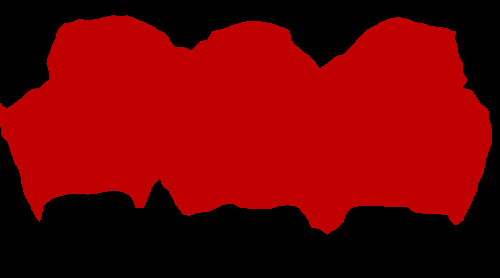
\includegraphics[height=0.10\linewidth]{fig/res_none/2008_001439.png} &
    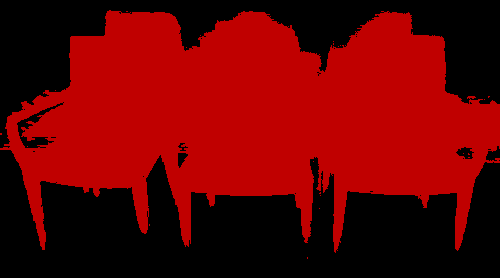
\includegraphics[height=0.10\linewidth]{fig/res_crf/2008_001439.png} &
    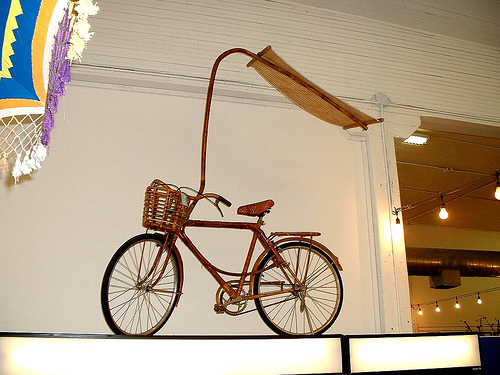
\includegraphics[height=0.12\linewidth]{fig/img/2008_004363.jpg} &
    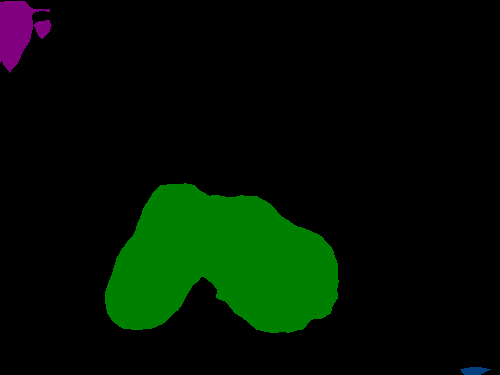
\includegraphics[height=0.12\linewidth]{fig/res_none/2008_004363.png} &
    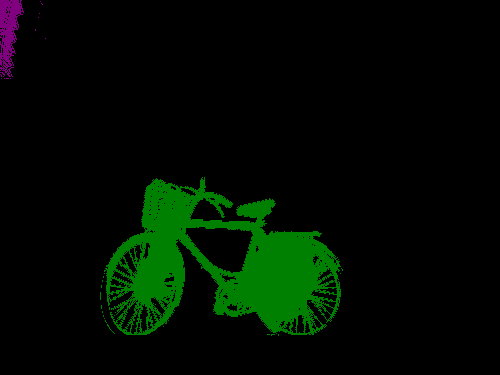
\includegraphics[height=0.12\linewidth]{fig/res_crf/2008_004363.png} \\
    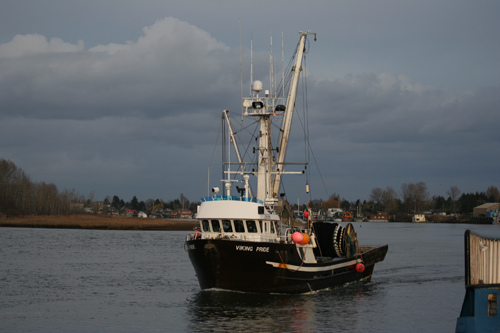
\includegraphics[height=0.12\linewidth]{fig/img/2008_006229.jpg} &
    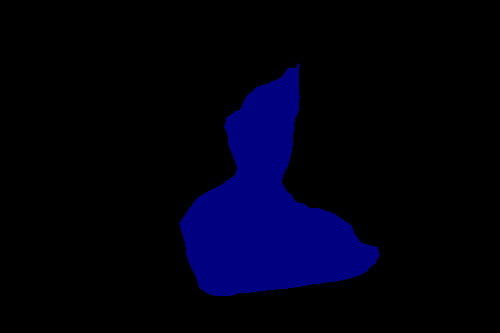
\includegraphics[height=0.12\linewidth]{fig/res_none/2008_006229.png} &
    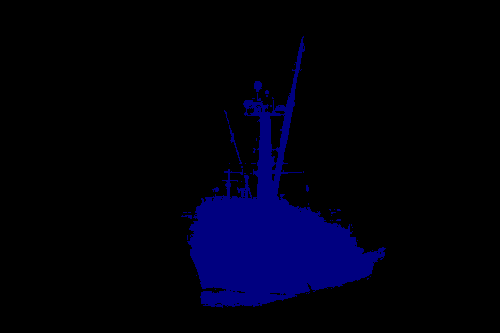
\includegraphics[height=0.12\linewidth]{fig/res_crf/2008_006229.png} &
    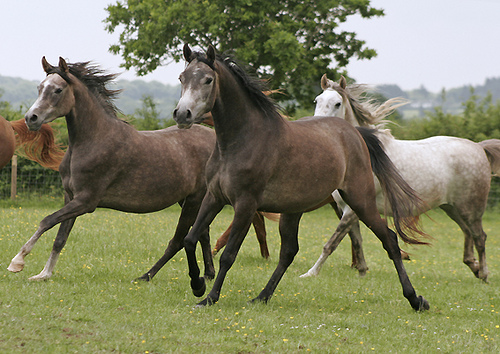
\includegraphics[height=0.12\linewidth]{fig/img/2009_000412.jpg} &
    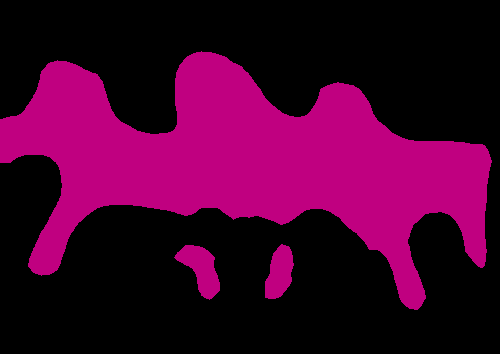
\includegraphics[height=0.12\linewidth]{fig/res_none/2009_000412.png} &
    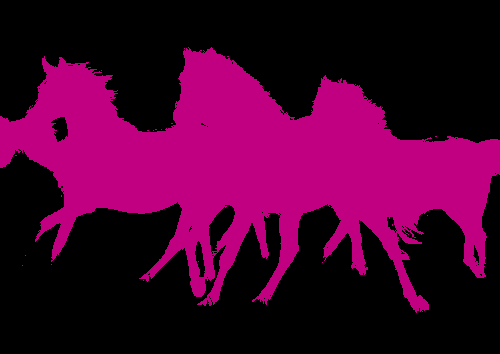
\includegraphics[height=0.12\linewidth]{fig/res_crf/2009_000412.png} \\
    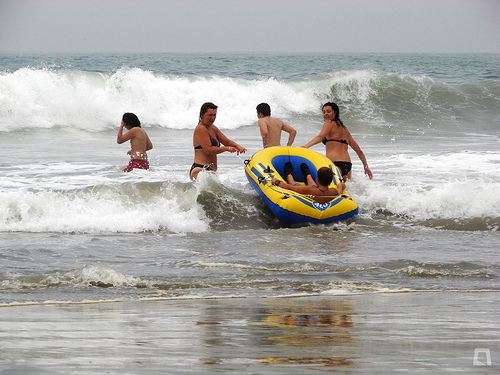
\includegraphics[height=0.12\linewidth]{fig/img/2009_000421.jpg} &
    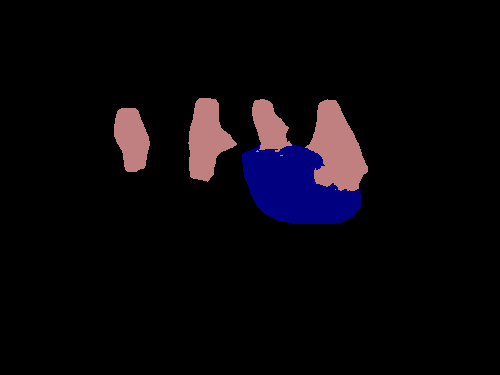
\includegraphics[height=0.12\linewidth]{fig/res_none/2009_000421.png} &
    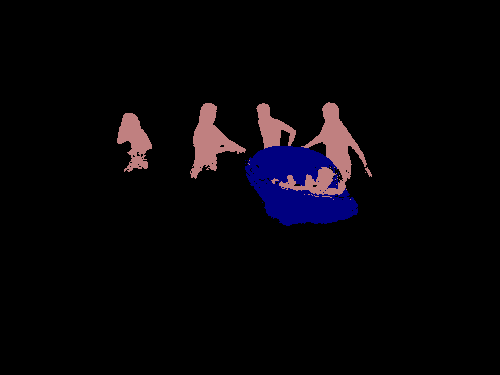
\includegraphics[height=0.12\linewidth]{fig/res_crf/2009_000421.png} &
    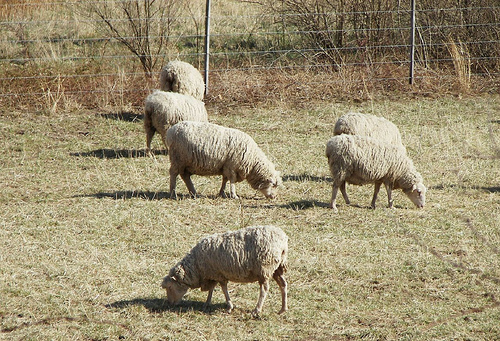
\includegraphics[height=0.12\linewidth]{fig/img/2010_001079.jpg} &
    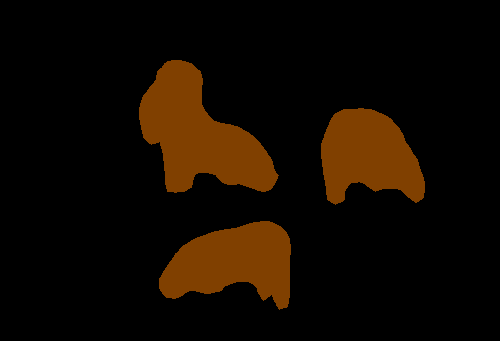
\includegraphics[height=0.12\linewidth]{fig/res_none/2010_001079.png} &
    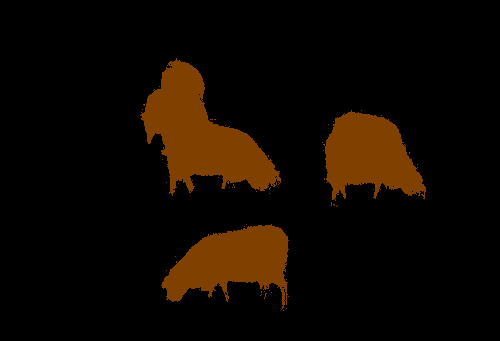
\includegraphics[height=0.12\linewidth]{fig/res_crf/2010_001079.png} \\
    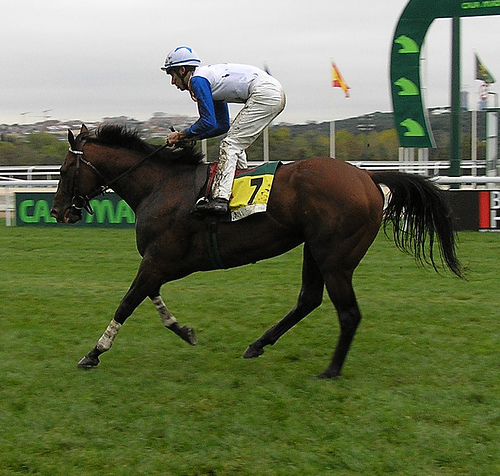
\includegraphics[height=0.12\linewidth]{fig/img/2010_000038.jpg} &
    \includegraphics[height=0.12\linewidth]{fig/res_none/2010_000038.png} &
    \includegraphics[height=0.12\linewidth]{fig/res_crf/2010_000038.png} &
    \includegraphics[height=0.12\linewidth]{fig/img/2010_001024.jpg} &
    \includegraphics[height=0.12\linewidth]{fig/res_none/2010_001024.png} &
    \includegraphics[height=0.12\linewidth]{fig/res_crf/2010_001024.png} \\
    \includegraphics[height=0.24\linewidth]{fig/img/2007_005331.jpg} &
    \includegraphics[height=0.24\linewidth]{fig/res_none/2007_005331.png} &
    \includegraphics[height=0.24\linewidth]{fig/res_crf/2007_005331.png} &
    \includegraphics[height=0.24\linewidth]{fig/img/2008_004654.jpg} &
    \includegraphics[height=0.24\linewidth]{fig/res_none/2008_004654.png} &
    \includegraphics[height=0.24\linewidth]{fig/res_crf/2008_004654.png} \\
    \includegraphics[height=0.24\linewidth]{fig/img/2007_000129.jpg} &
    \includegraphics[height=0.24\linewidth]{fig/res_none/2007_000129.png} &
    \includegraphics[height=0.24\linewidth]{fig/res_crf/2007_000129.png} &
    \includegraphics[height=0.24\linewidth]{fig/img/2007_002619.jpg} &
    \includegraphics[height=0.24\linewidth]{fig/res_none/2007_002619.png} &
    \includegraphics[height=0.24\linewidth]{fig/res_crf/2007_002619.png} \\
    \includegraphics[height=0.12\linewidth]{fig/img/2007_002852.jpg} &
    \includegraphics[height=0.12\linewidth]{fig/res_none/2007_002852.png} &
    \includegraphics[height=0.12\linewidth]{fig/res_crf/2007_002852.png} &
    \includegraphics[height=0.12\linewidth]{fig/img/2010_001069.jpg} &
    \includegraphics[height=0.12\linewidth]{fig/res_none/2010_001069.png} &
    \includegraphics[height=0.12\linewidth]{fig/res_crf/2010_001069.png} \\
    \hline
    \hline
    \includegraphics[height=0.12\linewidth]{fig/img/2007_000491.jpg} &
    \includegraphics[height=0.12\linewidth]{fig/res_none/2007_000491.png} &
    \includegraphics[height=0.12\linewidth]{fig/res_crf/2007_000491.png} &
    \includegraphics[height=0.12\linewidth]{fig/img/2007_000529.jpg} &
    \includegraphics[height=0.12\linewidth]{fig/res_none/2007_000529.png} &
    \includegraphics[height=0.12\linewidth]{fig/res_crf/2007_000529.png} \\
    \includegraphics[height=0.12\linewidth]{fig/img/2007_000559.jpg} &
    \includegraphics[height=0.12\linewidth]{fig/res_none/2007_000559.png} &
    \includegraphics[height=0.12\linewidth]{fig/res_crf/2007_000559.png} &
    \includegraphics[height=0.12\linewidth]{fig/img/2007_000663.jpg} &
    \includegraphics[height=0.12\linewidth]{fig/res_none/2007_000663.png} &
    \includegraphics[height=0.12\linewidth]{fig/res_crf/2007_000663.png} \\    
    \includegraphics[height=0.12\linewidth]{fig/img/2007_000452.jpg} &
    \includegraphics[height=0.12\linewidth]{fig/res_none/2007_000452.png} &
    \includegraphics[height=0.12\linewidth]{fig/res_crf/2007_000452.png} &
    \includegraphics[height=0.12\linewidth]{fig/img/2007_002268.jpg} &
    \includegraphics[height=0.12\linewidth]{fig/res_none/2007_002268.png} &
    \includegraphics[height=0.12\linewidth]{fig/res_crf/2007_002268.png} \\
  \end{tabular}
  }
  %\vspace{-0.3cm}
  \caption{Visualization results on VOC 2012-val. For each row, we show the input image, the segmentation result delivered by the DCNN, and the refined segmentation result of the Fully Connected CRF. We show our failure modes in the last three rows.} 
  \label{fig:ValResults}
\end{figure}
